% !TEX root = ../thesis.tex
% !TEX spellcheck = en-US

\clearpage

\section{Explorative Experiments with Paragraph Dataset}

\section{Experiments with Sentence Dataset}

\subsection{Vector Space Models compared}


\todo{say why using the sentence dataset here}
\todo{reference jupyter notebook here}
% http://localhost:8888/notebooks/thesis/experiments/vector-space-models/Vector%20Space%20Models.ipynb#Setup

As Section~\ref{sec:vector-space-models} explains, a popular way to approach text classification and other tasks in natural language processing is to build a language model by creating explicit representations of the objects or entities to be processed in a vector space. Such vectors can be used as features for a learning algorithm. Depending on the representation they can also further meaning, such as to encode notions of similarity of associativity between the objects.

In order to determine effective vector space representations for the task of sentence classification, a set of experiments was carried out to study and compare different approaches. Each method was studied with regards to the effect of its hyper-parameters on effectiveness when producing an input space to different classifiers, but also time and memory requirements at training and inference time are taken into account \todo{actually discuss time and memory requirements}.

In order to compare the effectiveness for the sentence classification task as discussed in ?\todo{reference section here} each labelled document was transformed into a vector space representation using the different methods and then used for classification with a simple logistic regression classifier (\todo{link to logistic regression classifier explanation here}). Performance was then compared with regards to Matthews Correlation Coefficient for multi-class problems \todo{link MCC multi here} and Accuracy.

\subsubsection{Baselines Classifiers: Uniform and Stratified Guessing}
\label{subs:baselines-classifiers}

As a baseline for comparing the performance of classification two different guessing strategies were used, namely uniform and stratified guessing.
Uniform guessing refers to a predictor that samples from the given classes assuming a uniform distribution whereas stratified guessing takes the label distribution in the data as the underlying probability distribution.
Then both methods just sample from these distributions to produce ``predictions'', while ignoring the actual input data. Both, uniform and stratified guessing achieve a Matthews Correlation Coefficient score of around 0 (averaged over 1000 runs) as expected for guessing strategies (see Section~\ref{subs:informedness-markedness-mcc}). On the other hand the accuracy for uniform guessing is around 0.16 which corresponds to $1/\text{K}$ for the K classes and around 0.26 for stratified guessing which reflects the skew of the label distribution.
Figure~\ref{fig:exp-vector-space-conf-matrix-guessing} shows the confusion matrices for these baseline variants in absolute and normalized form, revealing the properties of these guessing strategies.

\begin{figure}[h]
 % From http://localhost:8888/notebooks/thesis/experiments/vector-space-models/Vector%20Space%20Models.ipynb#Baseline:-Guessing-Strategies
    \centering
    \begin{subfigure}[b]{0.47\textwidth}
        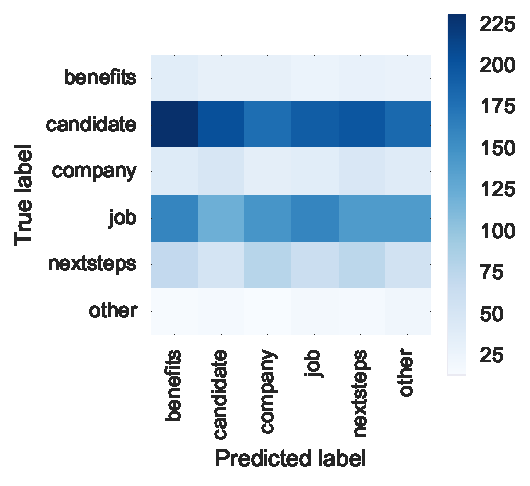
\includegraphics[width=\textwidth]{img/exp-vector-space-conf-matrix-guessing-uniform.pdf}
        \caption{Uniform, absolute}
    \label{fig:exp-vector-space-conf-matrix-guessing-uniform}
    \end{subfigure}
~
    %add desired spacing between images, e. g. ~, \quad, \qquad, \hfill etc.
    %(or a blank line to force the subfigure onto a new line)
    \begin{subfigure}[b]{0.48\textwidth}
        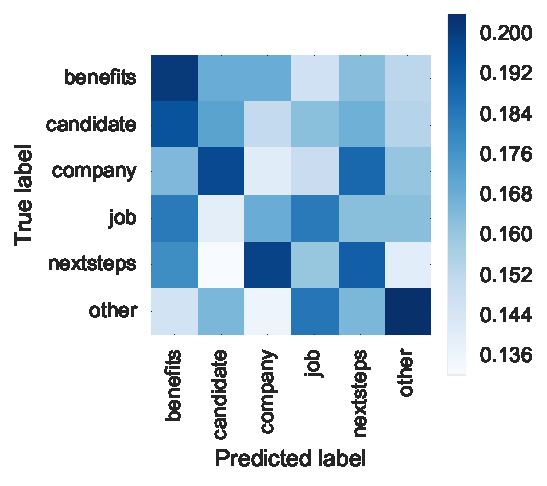
\includegraphics[width=\textwidth]{img/exp-vector-space-conf-matrix-guessing-uniform-normalized.pdf}
        \caption{Uniform, normalized}
      \label{fig:exp-vector-space-conf-matrix-guessing-uniform-normalized}
    \end{subfigure}
~
    \begin{subfigure}[b]{0.47\textwidth}
        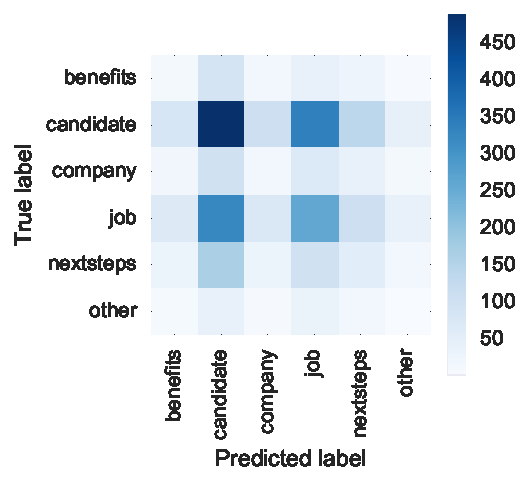
\includegraphics[width=\textwidth]{img/exp-vector-space-conf-matrix-guessing-stratified.pdf}
        \caption{Stratified, absolute}
      \label{fig:exp-vector-space-conf-matrix-guessing-stratified}
    \end{subfigure}
~
    %add desired spacing between images, e. g. ~, \quad, \qquad, \hfill etc.
    %(or a blank line to force the subfigure onto a new line)
    \begin{subfigure}[b]{0.48\textwidth}
        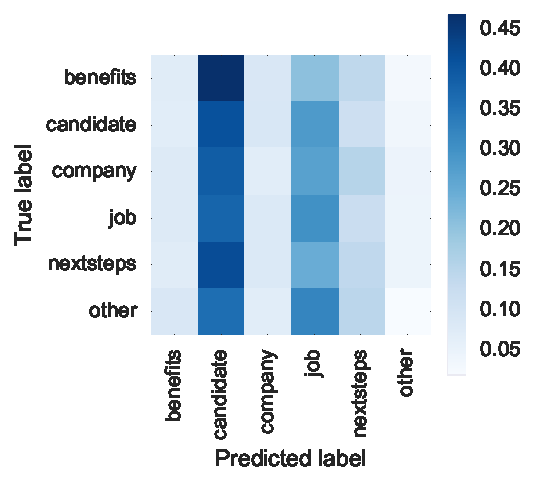
\includegraphics[width=\textwidth]{img/exp-vector-space-conf-matrix-guessing-stratified-normalized.pdf}
        \caption{Stratified, normalized}
      \label{fig:exp-vector-space-conf-matrix-guessing-stratified-normalized}
    \end{subfigure}
    \caption{Confusion matrices of uniform and stratified guessing strategies. }
\label{fig:exp-vector-space-conf-matrix-guessing}
\end{figure}

\subsubsection{N-gram Language Models}

The first class of language models that was investigated for the task of multi-class classification are N-gram models that were explained in Section~\ref{subs:n-gram-language-models}. As mentioned, in essence this type of model relies on simple statistics which makes for straightforward computation but at the same time comes at cost of expressiveness, especially in terms of temporal dependencies between words.

As N-grams models come in a variety of variants the most important ones were used as hyper-parameters to the model and a grid search was carried out over a wide range of combinations over these. The specific hyper-parameter settings are listed in Table~\ref{tab:ngram-parameters}. The grid search was optimized with regards to its \emph{multi-class log loss} (see section \todo{ref here}) while using it's resulting model for 5-fold cross-validated classification using Logistic Regression and Naive Bayes.

\begin{center}
  \begin{table}[h]
  \begin{tabular}{ l l l}
    \toprule
    Hyper-Parameter & N-gram Type: Words & N-gram Type: Characters \\
    \midrule
    N-gram Range (Range) & [1,1], [1,2], [1,3], [2,3], [3,3] & [1,5], [1,10], [5,10], [5,15] \\
    Stop Words & English, None & N/A \\
    Vector Size (Size) & 10, 100, 300 & 10, 100, 300 \\
    IDF & Yes, No & Yes, No \\
    Norm & L1, L2, None & L1, L2, None \\
    Sub-linear TF & Yes, No & Yes, No \\
    \bottomrule
  \end{tabular}
  \caption{Parameter search space word and character level N-gram models}
  \label{tab:ngram-parameters}
  \end{table}
\end{center}


\begin{center}
  \begin{table}[h]
  \begin{tabular}{ l l l l l l l l }
    \toprule
    Type & Range & Stop words & Size & IDF & Norm & Sub-linear TF & Log Loss \\
    \midrule
    Word & [1,1] & None & 300 & No & & Yes & -0.667 \\
    Word & [1,1] & None & 300 & No & & No & -0.669 \\
    Word & [1,2] & None & 300 & No & & Yes & -0.678 \\
    Word & [1,2] & None & 300 & No & & No & -0.681 \\
    Word & [1,3] & None & 300 & No & & Yes & -0.684 \\
    Word & [1,1] & None & 300 & Yes & L2 & Yes & -0.687 \\
    Word & [1,3] & None & 300 & No & & No & -0.687 \\
    Word & [1,1] & None & 300 & Yes & L2 & No & -0.688 \\
    Word & [1,2] & None & 300 & Yes & L2 & Yes & -0.693 \\
    Word & [1,2] & None & 300 & Yes & L2 & No & -0.694 \\
    \bottomrule
  \end{tabular}
  \caption{Top 10 results of grid search over hyper-parameter space as listed in Table~\ref{tab:ngram-parameters} using a 5-fold cross-validated Logistic Regression classifier}
\label{tab:ngram-grid-results-logreg}
  \end{table}
\end{center}

\begin{center}
  \begin{table}[h]
  \begin{tabular}{ l l l l l l l l }
    \toprule
    Type & Range & Stop words & Size & IDF & Norm & Sub-linear TF & Log Loss \\
    \midrule
    Word & 1,2 & None & 300 & Yes & l2 & Yes & -0.747 \\
    Word & 1,2 & None & 300 & Yes & l2 & No & -0.748 \\
    Word & 1,3 & None & 300 & Yes & l2 & Yes & -0.752 \\
    Word & 1,3 & None & 300 & Yes & l2 & No & -0.753 \\
    Word & 1,1 & None & 300 & Yes & l2 & Yes & -0.755 \\
    Word & 1,1 & None & 300 & Yes & l2 & No & -0.757 \\
    Word & 1,1 & English & 300 & No & l2 & Yes & -0.769 \\
    Word & 1,1 & English & 300 & No & l2 & No & -0.769 \\
    Word & 1,2 & None    & 300 & No & l2 & Yes & -0.77 \\
    Word & 1,2 & English & 300 & No & l2 & Yes & -0.772 \\
    \bottomrule
  \end{tabular}
  \caption{Top 10 results of grid search over hyper-parameter space as listed in Table~\ref{tab:ngram-parameters} using a 5-fold cross-validated Naive Bayes classifier}
\label{tab:ngram-grid-results-nb}
  \end{table}
\end{center}


\begin{center}
  \begin{table}[h]
  \begin{tabular}{ r | *3l | *3l }
    \toprule
     & \multicolumn{3}{c|}{Training} & \multicolumn{3}{|c}{Validation}\\
    Classifier & Log Loss & Accuracy & MCC & Log Loss & Accuracy & MCC \\
    \midrule
    Logistic Regression & 6.602 & 0.809 & 0.736 & 7.324 & 0.788 & 0.703 \\
    Naive Bayes         & 8.378 & 0.757 & 0.663 & 8.169 & 0.763 & 0.667 \\
    \bottomrule
  \end{tabular}
  \caption{Performance of each best N-gram model with Logistic Regression and Naive Bayes on the validation data}
\label{tab:ngram-grid-results-nb}
  \end{table}
\end{center}

\todo{Find out why the log loss here is so high (or why it's low in the CV)!! is it per class?}


\begin{figure}[h]
    \centering
    \begin{subfigure}[b]{0.47\textwidth}
        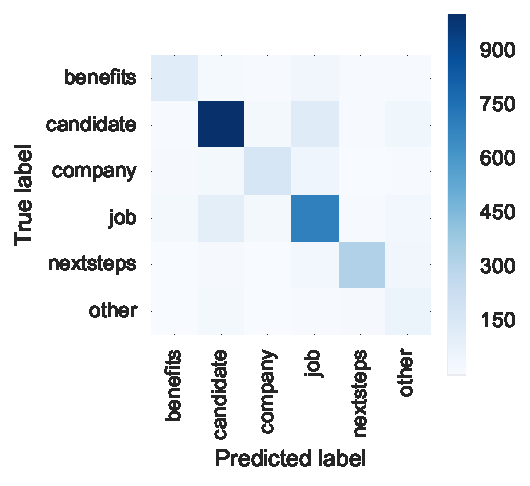
\includegraphics[width=\textwidth]{img/exp-vector-space-conf-matrix-logreg.pdf}
        \caption{Absolute}
        \label{fig:exp-vector-space-conf-matrix-logreg}
    \end{subfigure}
    ~
    %add desired spacing between images, e. g. ~, \quad, \qquad, \hfill etc.
    %(or a blank line to force the subfigure onto a new line)
    \begin{subfigure}[b]{0.48\textwidth}
        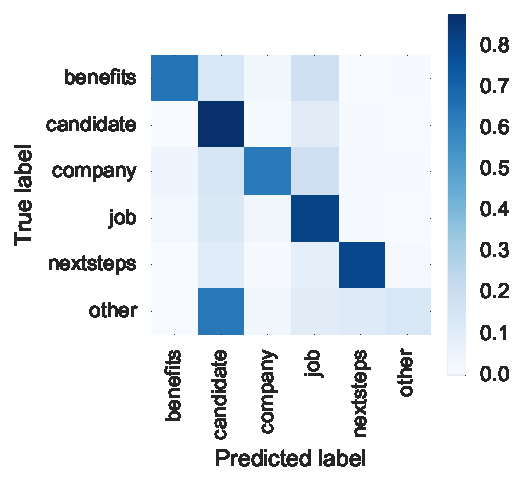
\includegraphics[width=\textwidth]{img/exp-vector-space-conf-matrix-logreg-normalized.pdf}
        \caption{Normalized}
        \label{fig:exp-vector-space-conf-matrix-logreg-normalized}
    \end{subfigure}
    \caption{Confusion matrix of logistic regression classifier using the best N-gram model found via cross-validated grid search}
  \label{fig:exp-vector-space-conf-matrix-guessing}
\end{figure}



\todo{show influence of each parameter on the performance by fixing it to each value it can take and measuring the variance of the results? or by just showing the mean when fixing to one value}

\subsubsection{Bag-of-Means -word2Vec averaged}

\subsubsection{Doc2Vec --- Distributed representations of documents}

\paragraph{Vector Size}

\paragraph{Frequeword Sub-Sampling}

\paragraph{Hierarchical Sampling}

\paragraph{Negative Sampling}

\paragraph{Window Size}

\paragraph{CBOW versus PM-DV}

\paragraph{Evaluating the best hyper-parameter setting}

\subsubsection{Doc2Vec using pre-initialized weights}

\subsubsection{Doc2Vec using context sentences}

\subsubsection{Results and Discussion}

\begin{figure}[h]
    \centering
    \begin{subfigure}[b]{0.47\textwidth}
      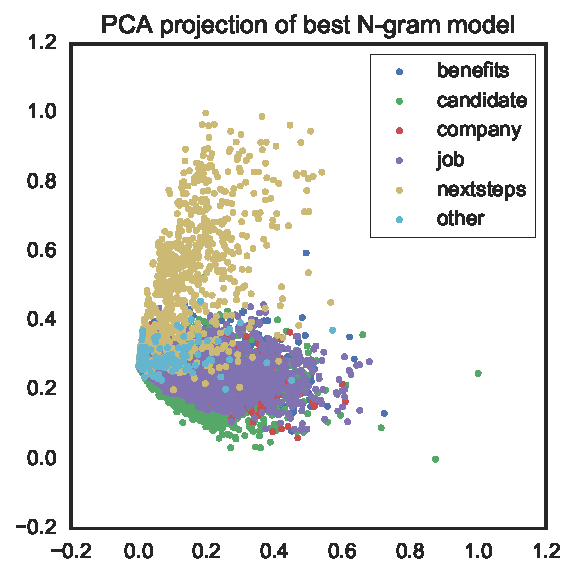
\includegraphics[width=\textwidth]{img/exp-vector-space-ngram-pca.pdf}
      \caption{PCA projection}
      \label{fig:exp-vector-space-ngram-pca}
    \end{subfigure}
    ~
    %add desired spacing between images, e. g. ~, \quad, \qquad, \hfill etc.
    %(or a blank line to force the subfigure onto a new line)
    \begin{subfigure}[b]{0.48\textwidth}
      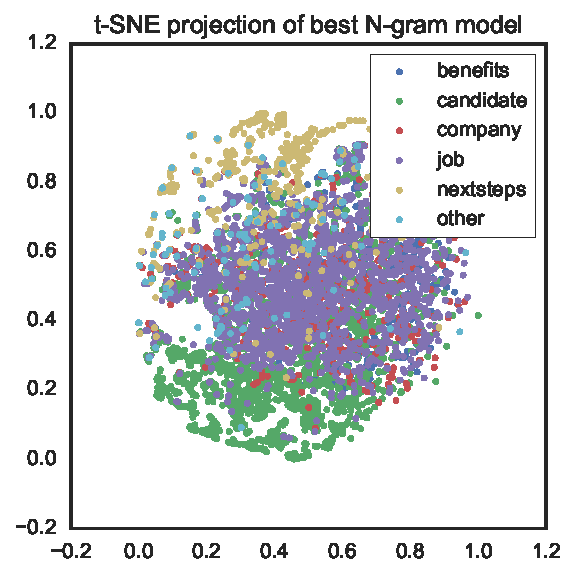
\includegraphics[width=\textwidth]{img/exp-vector-space-ngram-tsne.pdf}
      \caption{t-SNE projection}
      \label{fig:exp-vector-space-ngram-tsne}
    \end{subfigure}
    \caption{Document vectors produced by the best N-gram model (optimized w.r.t. Logistic Regression) projected onto the first 2 principal components}
  \label{fig:exp-vector-space-ngram}
\end{figure}



\subsection{Finding the best Classifier using Vector Space Models}

\subsection{Advanced and experimental approaches}

\subsubsection{Inversion of Distributed Language Representations}

\subsubsection{LSTM Multi-task learner}
\label{subs:LSTM Multi-task learner}
